
\chapter{Методы моделирования ондуляторного излучения от пучка с конечным эмиттансом} \label{chapt2}
\rr{интро}
\rr{сделать обзор литературы по тому какие подходы в основном реализуются сейчас: Гаусс-Шелл модель, указать на несоответствие того, что ондуляторное излучение имеет форму синк-функции}

\section{О статистических свойствах синхротронного излучения}
Электромагнитное излучение от электронного пучка с конечным эмиттансом может быть представлено как сумма полей от каждого индивидуального электрона. Каждый $k$ электрон в пучке имеет свою координату -- $\vec{\eta}_k$, угол -- $\vec{\l}_k$, отсчитываемые от проектной траектории, а также продольную координату или, другими словами, время прибытия $t_k$ относительно некоторого времени $t_0$, вклад которого в $r\omega$-пространстве будет умножением поля на фазовый фактор $\exp{(i \omega t_k)}$. Указанные величины подчиняются некоторым распределениям плотности вероятности, для накопительных колец в модельных случаях это распределение Гаусса. В данном случае не рассматривается разброс электронов по энергии, он будет включён в рассмотрение позже. Объём фазового пространства, который составляют эти шесть переменных, и есть эмиттанс электронного пучка. Результирующее поле от $N_e$ электронов можно записать следующим образом:
\begin{align}
	\bar{E}_{b} (z, \vec{r}, \omega) = \sum\limits_{k=1}^{N_e} \bar{E}(\vec{\eta}_k, \vec{\l}_k, z, \vec{r}, \omega) \exp{(i \omega t_k)},
	\label{eq:E_bunch} 
\end{align}
Для электронов в накопительных кольцах случайные величины $\vec{\eta}_k$ и $\vec{\l}_k$ не зависят от времени прибытия $t_k$. Модуля поля $\bar{E} = |\bar{E}_k|\exp{i\phi_k}$ имеет независящей от $k$ одинаковое распределение со средним $\big \langle|\bar{E}_k|\big \rangle$ и конечным вторым моментом  $\big \langle|\bar{E}_k|^2\big \rangle$. \rr{Всё это здорово, но должно откуда-то следовать. По всей видимости, эти предположения следуют из наличия дробового шума в электронном пучке (затухание и квантовая раскачка бетатронных колебаний). Нужна объяснительная команда.}.

Результирующее поле $\bar{E}_{b}$ является суммой вкладов от каждого электрона в пучке и по своей структуре в правой части уравнения~\ref{eq:E_bunch} записан некоторый фазор. Следуя предпосылкам центральной предельной теоремы (ЦПТ), можно показать, что $\bar{E}_{b}$ комплексная Гауссова переменная. Другими словами, амплитуда поля в каждой точке $\vec{r}$ подчиняется гауссовому распределению. Однако, предпосылки ЦПТ выполняются для двух практически значимых предельных случаев: случай длинного $\omega\sigma_T \gg 1$ и короткого электронного пучка $\omega\sigma_T \gg 1$, где $\sigma_T$ -- длительность электронного пучка \rr{а что не так с $\omega\sigma_T \sim 1$?}. В случае длинного электронного пучка величина $\omega t_k$ равномерно распределена в пределах от $0$ до $2\pi$ и излучение продольно некогерентно, для короткого пучка фазовый множитель $\exp{(i \omega t_k)}$ может быть взят равным единице и излучения является продольно когерентным. 

\section{Численное моделирование ондуляторного излучения}
Формула~\ref{eq:E_bunch} используется напрямую при моделирования ондуляторного излучения, как продольно когерентного так и некогерентного. Общий вид поля ондуляторного излучения от одного электрона с некоторыми углом $\vec{\eta}_k$ и координатой $\vec{\l}_k$ может быть записан как \cite{geloni_fourier_2007} \rr{спросить Джанлуку про эту формулу}: 
\begin{align}
	\bar{E}_{\bot}(z_0, \omega, \vec{\eta}_k, \vec{\l}_k, \vec{\theta} \;) =
&	-\frac{\omega e A_{JJ} L_s}{2c^2z_0}\frac{K}{\gamma}\exp{\bigg[i \frac{\omega z_0}{2c} \bigg|\vec{\theta} - \vec{\l}/z_0\bigg|^2 \bigg]} \cr & \times \sinc \bigg[\bigg(k_w \frac{\Delta \omega}{\omega} + \frac{\omega |\vec{\theta} - (\vec{\l}/z_0) - \vec{\eta}|^2}{2c}\bigg)\cfrac{L_s}{2}\bigg],
	\label{eq:single_electron_far_field}
\end{align}
где $\vec{\theta} = \vec{r}/z_0$ \rr{пояснить все новые параметры}. Формула \ref{eq:single_electron_far_field} даёт распределение амплитуды поля в дальней зоне ($z_0 \gg L_w$\rr{и что-то ещё}). Чтобы получить более точно выражение это поле должно быть отпропагировано назад в центр ондулятора с помощью пропагатора свободного пространства. Распределение поля в мнимом источнике излучения: \rr{Откуда взялась информация, которой не было. Нужна пояснительная команда.}
\begin{align}
	\widetilde{E}_{\bot}(0, \vec{\eta}, \vec{\l}, \vec{r}_{\bot}) =
	i \frac{e A_{JJ} \omega}{2 c^2}\frac{K}{\gamma} &\exp{\big[i \frac{\omega}{c} (\vec{r}_{\bot} - \vec{l})\big]}\cr & \times \bigg [\pi - 2\text{Si} \bigg( \cfrac{i \omega |\vec{r}_{\bot} - \vec{l}|^2}{L_w c}\bigg)\bigg], 
	\label{eq:single_electron_near_field_z=0}
\end{align}
после этого поле можно распространять на любую дистанцию вдоль оптической оси $z_0$. Снова применяя пропагатор свободно пространства, получаем:
\begin{align}
	\bar{E}_{\bot}(&z_0, \omega, \vec{\eta}_k, \vec{\l}_k, \vec{r}) =
		\frac{e A_{JJ} \omega}{2 c^2}\frac{K}{\gamma} \exp{\bigg[i \frac{\omega}{2 z_0 c} (|\vec{r}_{\bot} - \vec{l}|^2 - |\vec{r}_{\bot} - \vec{l} - z_0 \vec{\eta}|^2) \bigg]} \cr & \times	\bigg \{ \text{Ei} \bigg[ \cfrac{i \omega (\vec{r}_{\bot} - \vec{l} - z_0 \vec{\eta})^2}{2z_0c - L_w c}\bigg] - \text{Ei} \bigg[ \cfrac{i \omega (\vec{r}_{\bot} - \vec{l} - z_0 \vec{\eta})^2}{2z_0c + L_w c} \bigg] \bigg\}.
	\label{eq:single_electron_near_field}
\end{align}
Рассчитанное таким образом поле может быть рассчитано для любого значения $z_0$, такое поле называют поле в приближении ближней зоны, так как эта формула применим для значение $z_0 \sim L_w$. Обе формулы \ref{eq:single_electron_far_field} и \ref{eq:single_electron_near_field} имеют практическую ценность при моделировании, однако при использовании выражения \ref{eq:single_electron_near_field} время на моделирование значительно увеличивается, так как необходимо дважды численно взять интеграл $\textup{Ei}(\cdot)$.
 
После расчёта суммарного поля c $N_e$ электронами получившиеся монохроматическое поле по своей сути есть одна статистическая реализация поля. \rr{переформулировать следующее предложение} Физически это значит следующее, если экспериментатор измерит распределение интенсивности поля на детекторе от пролёта одного электронного пучка, используя монохроматор с разрешением, которое позволит разрешить одну продольную моду излучения, то на детекторе будет распределение эквивалентное по своим статистическим свойствам распределению, представленному на Рис.. 

После усреднения по $N_b$ реализациям (с идеальным монохроматором\footnote{другими словами, монохроматором разрешается одна поперечная мода}), наблюдаемая интенсивность даётся выражением: 
\begin{align}
	I_{\omega} = \bigg \langle \bigg|\sum\limits_{k=1}^{N_e} \bar{E}(\vec{\eta}_k, \vec{\l}_k, z, \vec{r}, \omega) \exp{(i \omega t_k)}\bigg|^2 \bigg \rangle,
	\label{eq:I_MC} 
\end{align}
\begin{figure}[H] 
	\centering 	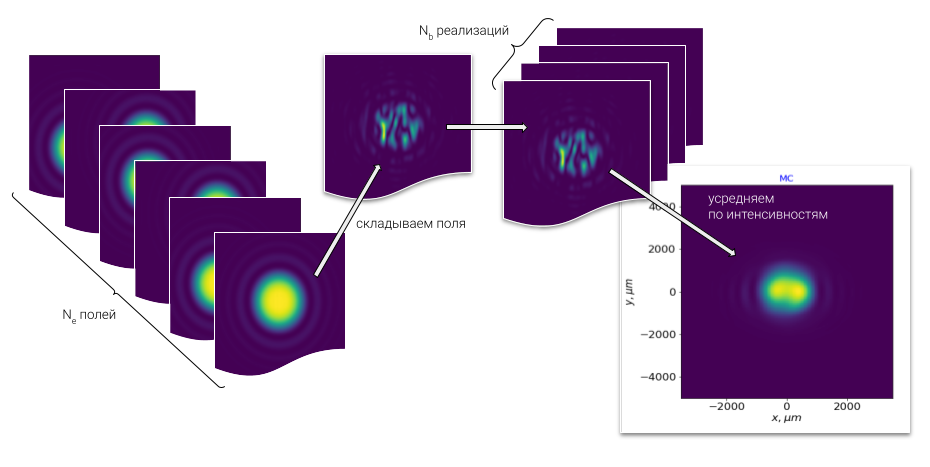
\includegraphics[width=0.99\linewidth]{MC_scheme.png}
	\caption{Схема работы метода сложения амплитуд \rr{перерисовать, изменить подпись}}
	\label{fig:SRW_scheme}
\end{figure}
\noindent результирующая интенсивность будет сходиться к некоторой огибающей. В грубом приближении огибающая является свёрткой распределения расходимости излучения и распределения расходимости электронного пучка. Данный подход является наиболее прямым подходом к задаче моделирования частично когерентного излучения, однако время расчёта в таком случае может быть оценено как время затрачиваемое на расчёт одной одного поля $N_e$ раз по формуле~\ref{eq:single_electron_far_field} или~\ref{eq:single_electron_near_field}, в последней, как уже упоминалось, необходимо дважды численно взять интеграл $\textup{Ei}(\cdot)$ и потом усреднить по $N_b$ реализациям поля $\bar{E}_{b}$. Итого, если за $\tau_{calc}$ взять время расчёта одного поля, то расчёт одного результирующего поля в сумме займёт $T_{calc} = \tau_{calc} \cdot N_e \cdot N_b$.

Однако в случае полностью некогерентного излучения время расчёта можно сократить за счёт фазового фактора $\exp{(i \omega t_k)}$, который эффективно приводит к тому, что отдельный электрон в электронном пучке коррелирует только с самим собой \cite{geloni_transverse_2008}. Таким образом формула~\ref{eq:I_MC} упрощается до 
\begin{align}
 	I_{\omega} = \sum\limits_{k=1}^{N_e} \bigg|\bar{E}(\vec{\eta}_k, \vec{\l}_k, z, \vec{r}, \omega)\bigg|^2,
 	\label{eq:I_SRW} 
\end{align}
\begin{figure}[H] 
	\centering 	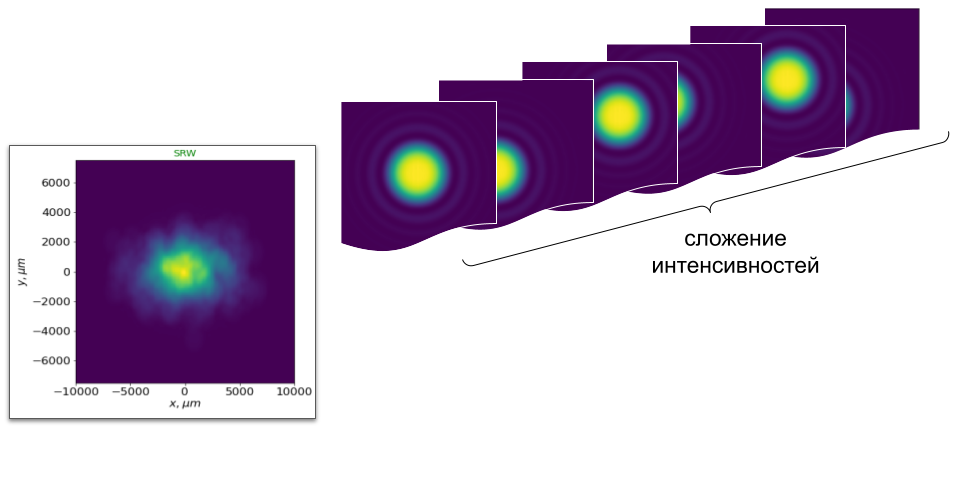
\includegraphics[width=0.99\linewidth]{SRW_scheme.png}
	\caption{Схема метода сложения интенсивностей \rr{перерисовать, изменить подпись}}
	\label{fig:SRW_scheme}
\end{figure}
\noindent а время расчёта уменьшается до $T_{calc} = \tau_{calc} \cdot N_e$. Недостатком такого подхода можно считать потерю фазовой информации о излучение и, следовательно, невозможности расчёта поперечной автокрелляционной функции первого порядка \rr{Можно ли через второй порядок найти первый? Нужна пояснительная команда}. Тем не менее, подход основанный на формуле~\ref{eq:I_SRW} даёт мощный метод расчёта частично когерентного излучения. Именно этот подход реализован в широко распространённом коде SRW \rr{cite}.
 
\subsection{Влияние размера электронного пучка на расходимость излучения}
\rr{где такой эффект можно неожиданно встретить?}

\rr{когерентный случай}
\begin{figure}[H] 
	\centering 	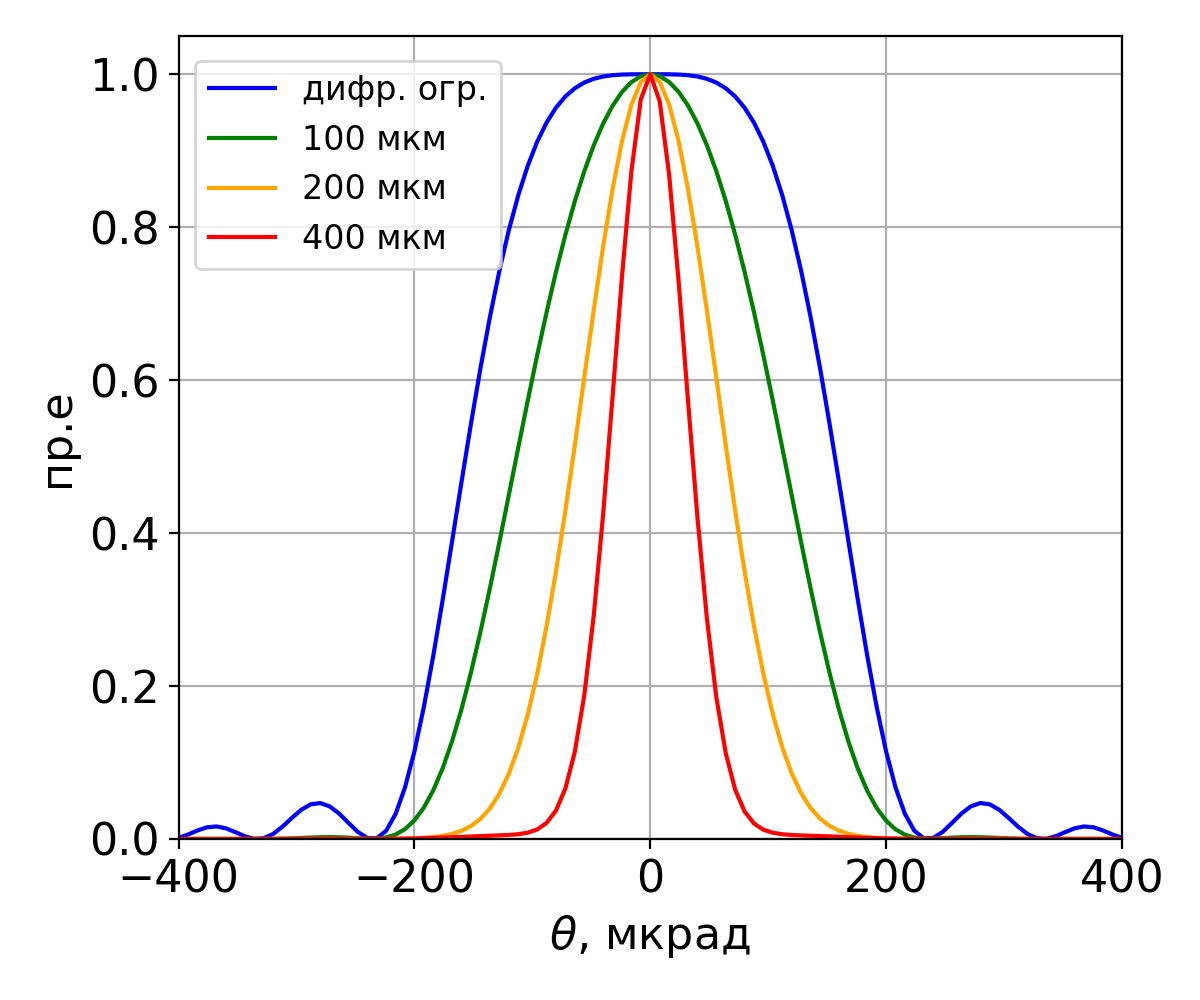
\includegraphics[width=0.99\linewidth]{diff_divergence_coh.png}
	\caption{Интенсивность комплексного гауссового шума}
	\label{fig:diff_coh_incoh_rad}
\end{figure}

\rr{некогерентный случай}
\begin{figure}[H] 
	\centering 	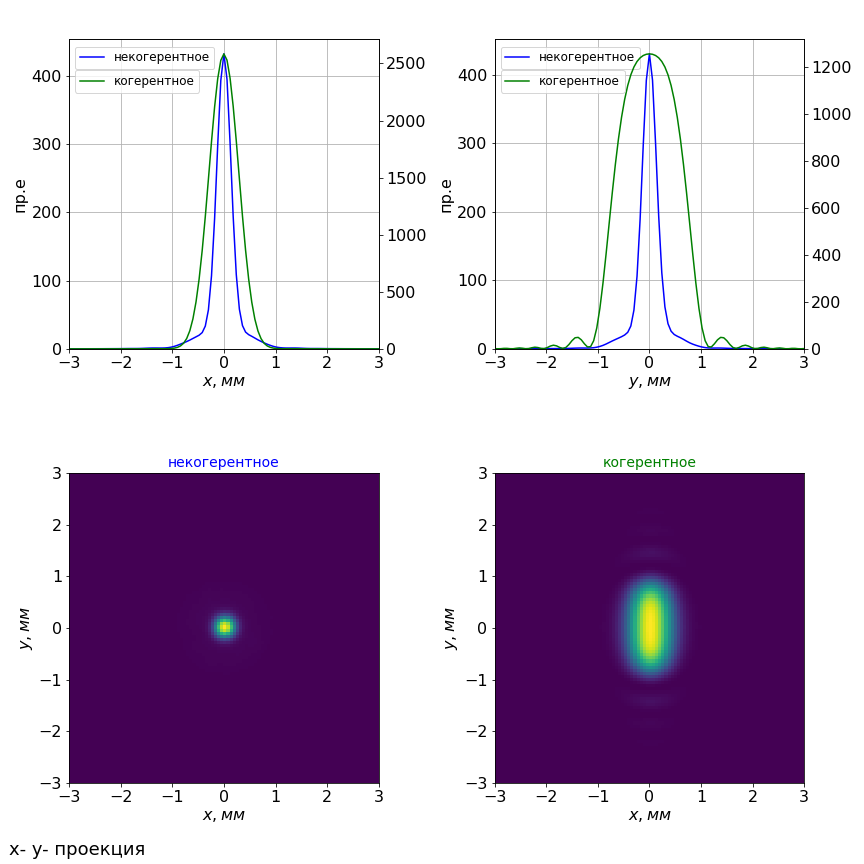
\includegraphics[width=0.99\linewidth]{diff_divergence_incoh.png}
	\caption{Интенсивность комплексного гауссового шума}
	\label{fig:diff_coh_incoh_rad}
\end{figure}

\subsection{Различие расходимости излучения для случая продольно полностью когерентного и некогерентного пучка}
В зависимости от длительности электронного пучка результирующее поле $\bar{E}_{b}$ будет вести себя по-разному. В случае короткого электронного пучка: $\omega \sigma_T \ll 1$, где $\sigma_T$ -- длительность электронного сгустка, излучение будет продольно когерентным, в иностранной литературе этот эффект называется Coherent Synchrotron Radiation (CSR). Методы моделирования такого излучения рассмотрены в работах \rr{cite}. Приближение короткого электронного пучка справедливо для низких энергий \rr{каких?}. Случай длинного электронного пучка, а именно  $\omega \sigma_T \gg 1$ соответствует случаю продольно некогерентного излучения, а для уравнения~\ref{eq:E_bunch} это означает, что показатель экспоненты $\omega \sigma_T$ равномерно распределён в интервале от $0$ до $2 \pi$. 

\rr{отличие на $\sqrt{2}$}

\rr{где такой эффект можно неожиданно встретить?}
\begin{figure}[H] 
	\centering 	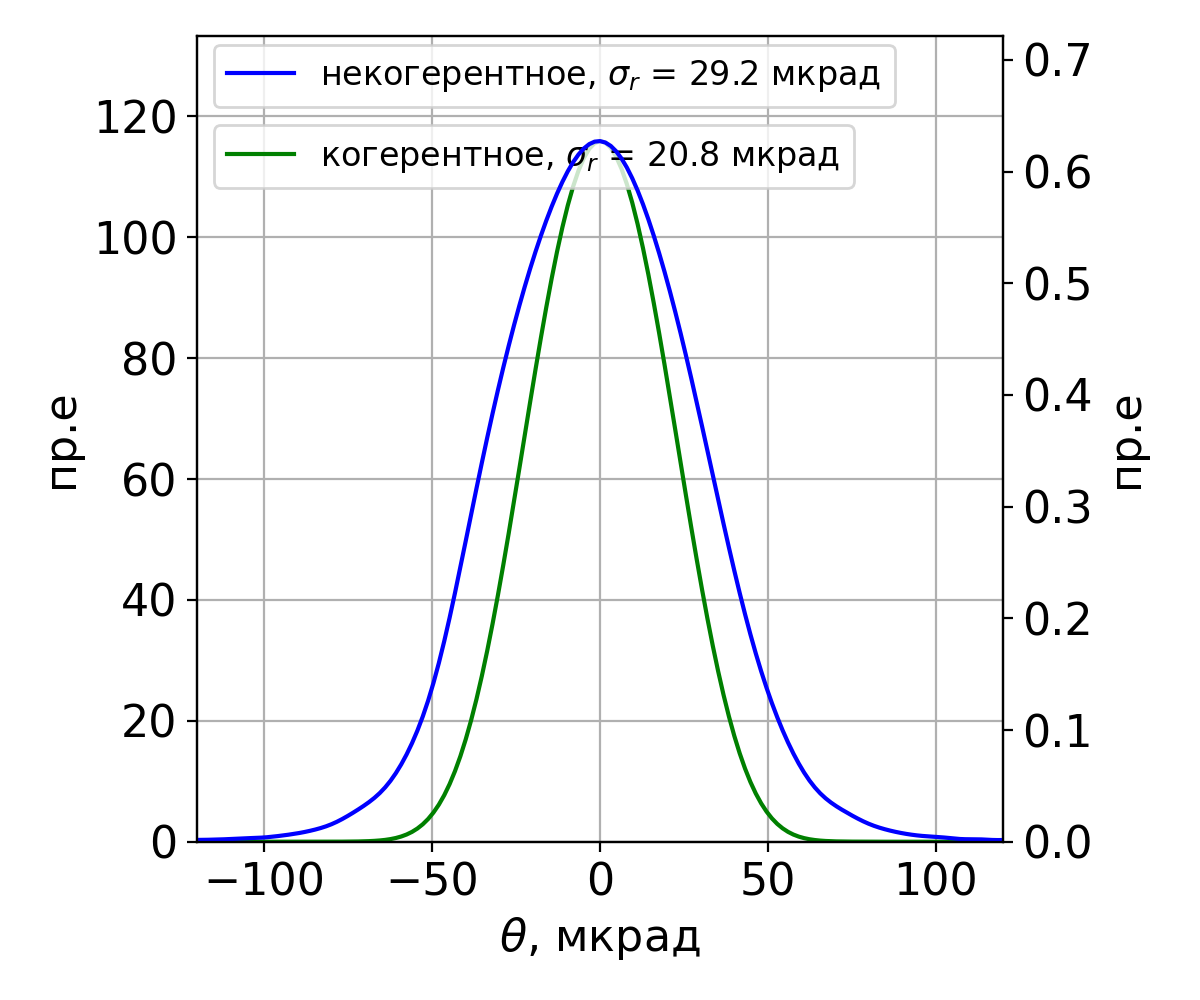
\includegraphics[width=0.99\linewidth]{diff_coh_incoh_rad.png}
	\caption{Интенсивность комплексного гауссового шума}
	\label{fig:diff_coh_incoh_rad}
\end{figure}
\subsection{Влияние энергетического разброса электронного пучка на расходимость излучения}
\rr{Как-то влияет}\\
\rr{картинки моделирования}
\section{Метод ограничения пространственных гармоник огибающими: SERVAL}
В работе предлагается эффективный метод для моделирования частично когерентного излучения, основанный на ограничении пространственного шума огибающими поля. Метод заключается в имитации дробового шума в электронном пучке комплексным Гауссовым шумом и последующим его ограничением пространственных мод этого шума эффективным размером и расходимостью электромагнитного поля в источнике. Эффетивный размер и расходимость поля оценивается как соответствующая свёртка распределения электронного пучка с распределением поля от электронного пучка с бесконечно малым поперечным эмиттансом в источнике излучения -- центре ондулятора. Выбор позиции в центре ондулятор объясняется тем, что ондуляторное излучение имеет плоский волновой фронт именно в центре ондулятора, этим оно схоже лазерными Гауссовыми пучками.

\subsection{Алгоритм получения поля}
Для начала алгоритм будет представлен в общем виде, без уточнения чем определяются распределение размера и расходимости излучения и, в целом, без относительно характера источника излучение -- в нашёл случае ондулятора. 
\begin{enumerate}
\item Создание комлексного гауссового шума $Z = X + iY$ в $r\omega$-пространстве, где величины $X$ и $Y$ подчиняются нормальному распределению.
\begin{figure}[H] 
	\centering 	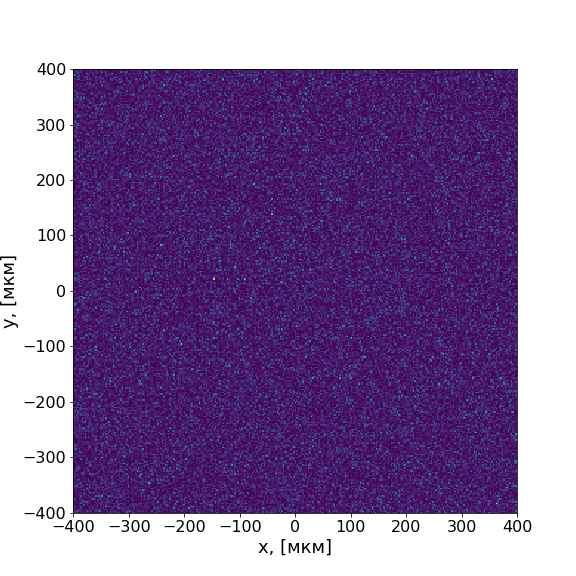
\includegraphics[width=0.45\linewidth]{1-X_noise.png}
	\caption{Интенсивность комплексного гауссового шума}
	\label{fig:1-noise}
\end{figure}
\item Ограничение шума эффективным размером электромагнитного излучения в \rr{перетяжке}.
\begin{figure}[H]
	\centering
	\begin{minipage}{0.45\textwidth}
		\centering
		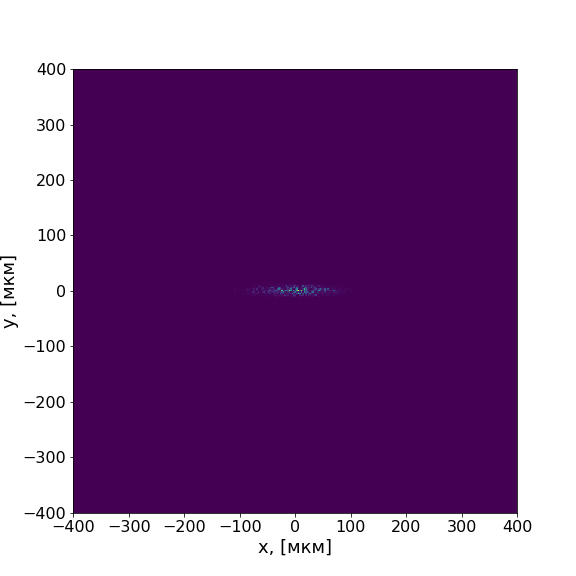
\includegraphics[width=1\linewidth]{2-X_e-beam-size.png}
		\caption{Размер электромагнитного излучения в перетяжке наложенный на шум}
		\label{fig:2-beam_size_k}
	\end{minipage}
	\begin{minipage}{0.45\textwidth}
		\centering
		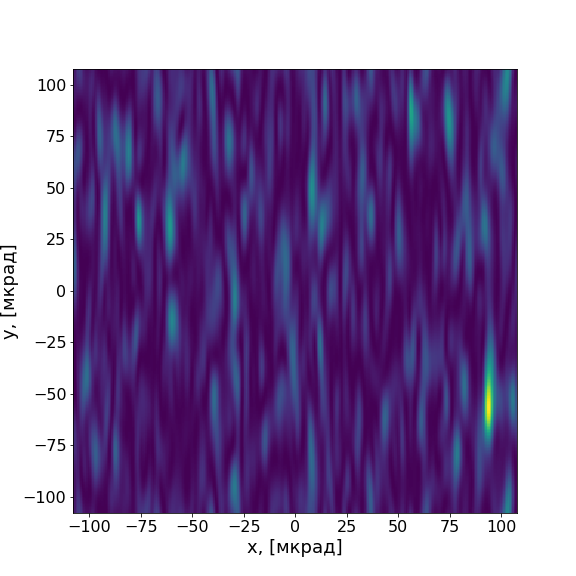
\includegraphics[width=1\linewidth]{2-X_e-beam-divergence.png}
		\caption{Получившиеся моды в $k\omega$-пространстве от размера электронного пучка}
		\label{fig:2-beam_size_s}
	\end{minipage}\hfill
\end{figure}
\item Ограничение пространственных мод эффективной расходимостью излучения
\begin{figure}[H]
	\centering
	\begin{minipage}{0.45\textwidth}
		\centering
		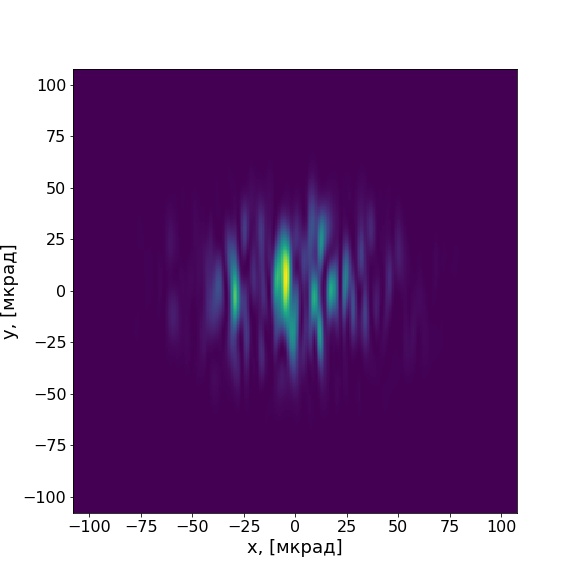
\includegraphics[width=1\linewidth]{3-X_radaition_divergence.png}
		\caption{Расходимость излучения}
		\label{fig:3-beam_s}
	\end{minipage}
	\begin{minipage}{0.45\textwidth}
		\centering
		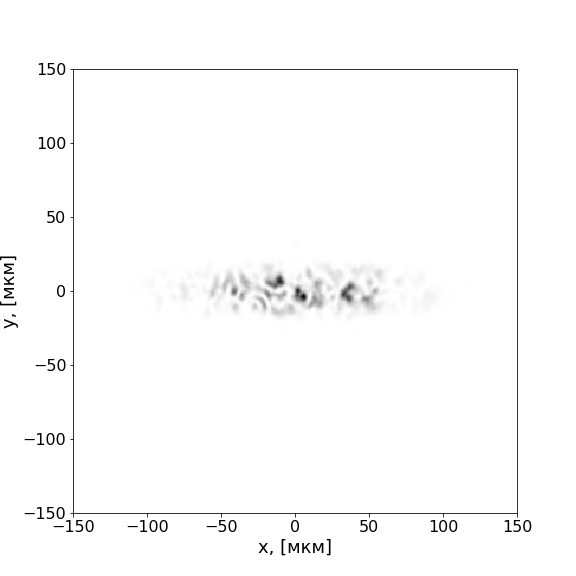
\includegraphics[width=1\linewidth]{3-X_radaition_size.png}
		\caption{Размер излучения в источнике}
		\label{fig:3-beam_k}
	\end{minipage}
\end{figure}
\item Распространение излучения через оптическую систему
\end{enumerate}

\subsection{Выбор подходящих огибающих}
При выполнение второго шага выполняется операция умножения шума, на распределение размера излучения. Размер излучения в случае электронного пучка с бесконечно малым поперечным эмиттансом может быть получено, как обратная пропагация излучения в дальней зоне~\ref{eq:single_electron_far_field} обратно в центр ондулятора посредствам пропагатора в свободном пространстве. Выражение для распределения поля в центре ондулятора даётся выражением:
\begin{align}
	\widetilde{E}_{\bot}(0, \vec{\eta}, \vec{\l}, \vec{r}_{\bot}) =
	i \frac{e A_{JJ} \omega}{2 c^2}\frac{K}{\gamma} &\exp{\big[i \frac{\omega}{c} (\vec{r}_{\bot} - \vec{l})\big]}\cr & \times \bigg [\pi - 2\text{Si} \bigg( \cfrac{i \omega |\vec{r}_{\bot} - \vec{l}|^2}{L_w c}\bigg)\bigg]
	\label{eq:single_electron_with_offset_and_tilt_near_field_z=0}
\end{align}
Для того, чтобы получить распределение амплитуды (интенсивности) излучение в случае электронного пучка с конечным эмиттансом следует произвести свёртку распределение размера электронного пучка $f(\vec{r})$ с распределением излучения амплитуды (интенсивности) от пучка с бесконечно малым эмиттансом. 
\begin{align}
	\bar{A}_{b} (0, \vec{r}) = \big(\widetilde{A}_{\bot}(0, 0, 0, \vec{r}_{\bot}) \ast f(\vec{r}_{\bot})\big), 
\end{align} 
тоже для шага 3. для расходимости.
\begin{align}
	\hat{\bar{A}}_{b} (0, \vec{\theta}, \omega) = \big(\hat{\widetilde{A}}_{\bot}(0, 0, 0, \vec{\theta}_{\bot}) \ast \hat{f}(\vec{\theta}_{\bot})\big), 
\end{align} 
именно $\bar{A}_{b} (0, \vec{r})$ и $\hat{\bar{A}}_{b} (0, \vec{\theta}, \omega)$ используются при ограничении пространственных гармоник огибающими. Однако, точный вид огибающих пока не затрагивался, а именно следует ли использовать в качестве свёртываемых функций амплитудные распределения, распределения интенсивности или же третий вариант квадратный корень из квадратов амплитуд.

\begin{enumerate}[label=\Roman*.]
	\item \label{ampl} $\bar{A}_{b} (0, \vec{r}) = \big(\widetilde{E}_{\bot}(0, 0, 0, \vec{r}_{\bot}) \ast f(\vec{r}_{\bot})\big)$
	
	$\hat{\bar{A}}_{b} (0, \vec{\theta}) = \big(\hat{\widetilde{E}}_{\bot}(0, 0, 0, \vec{\theta}_{\bot}) \ast \hat{f}(\vec{\theta}_{\bot})\big)$\\

	\item \label{square} $\bar{A}_{b} (0, \vec{r}) = \sqrt{\big(\widetilde{E}^2_{\bot}(0, 0, 0, \vec{r}_{\bot}) \ast f^2(\vec{r}_{\bot})\big)}$
	
	$\hat{\bar{A}}_{b} (0, \vec{\theta}) = \sqrt{\big(\hat{\widetilde{E}}^2_{\bot}(0, 0, 0, \vec{\theta}_{\bot}) \ast \hat{f^2}(\vec{\theta}_{\bot})\big)}$\\
	
	\item \label{mod} $\bar{A}_{b} (0, \vec{r}) = \big(\big|\widetilde{E}_{\bot}(0, 0, 0, \vec{r}_{\bot})\big| \ast f(\vec{r}_{\bot})\big)$
	
	$\hat{\bar{A}}_{b} (0, \vec{\theta}) = \big(\big|\hat{\widetilde{E}}_{\bot}(0, 0, 0, \vec{\theta}_{\bot})\big| \ast \hat{f}(\vec{\theta}_{\bot})\big)$\\
\end{enumerate}
Чтобы выбрать для каждого из случаев наиболее подходящую огибающую проще всего проверить поведение поля в обычной фокусирующей системе, каким образом поле выглядит в дальней зоне и после фокусировки в фокальной плоскости. Сравнив поля, рассчитываемые методом SERVAL с наиболее реалистичным методом, основанным на подходе Монте-Карло будет сделан вывод о применимости огибающих \ref{ampl}, \ref{square} и \ref{mod} 

\rr{картинки различных распределений в случае почти когерентного источника в одном направлении и некогерентного источника в другом}

\section{Сравнение метода Монте-Карло, SRW и SERVAL}

\subsection{Дифракция на апертуре}

\subsection{Фокусировка}

\subsection{Фокусировка сферическим зеркалом с шероховатостями}








